\documentclass{beamer}
\usetheme{Madrid}
\usecolortheme{default}
\setbeamertemplate{navigation symbols}{}
\usepackage{tikz}
\usetikzlibrary{positioning,arrows.meta}

\title{Agentic Workflow for Automated Binary/APK Analysis}
\author{Abdeljalil Otman}
\date{March 22, 2026}

\begin{document}

\begin{frame}
  \titlepage
\end{frame}

\begin{frame}{Problem Statement}
  \begin{itemize}
    \item Malware analysis is multi-stage and tool-heavy, especially across binaries and APKs.
    \item Analysts need consistent, high-level signals rather than raw tool output.
    \item Modern malware uses obfuscation and packing, making triage slower.
  \end{itemize}
\end{frame}

\begin{frame}{Objectives}
  \begin{itemize}
    \item Build MCP tools with high-level analysis abstractions.
    \item Orchestrate tools with an LLM agent (Agno) for concise risk summaries.
    \item Provide CLI, JSON reports, and containerized execution.
    \item Operate under low-resource constraints with minimal dependencies.
  \end{itemize}
\end{frame}

\begin{frame}{Agenda}
  \begin{itemize}
    \item Architecture and tool design
    \item Analysis coverage (binary + APK)
    \item Evaluation protocol and results
    \item Limitations and future work
  \end{itemize}
\end{frame}

\begin{frame}{Architecture}
  \begin{columns}[T]
    \begin{column}{0.52\textwidth}
      \begin{block}{Pipeline}
        \texttt{CLI $\to$ Agno Agent $\to$ MCP Servers}\\
        \texttt{$\quad$ (Static/Dynamic/Pattern/APK)}\\
        \texttt{$\quad$ $\to$ Analysis Backends}
      \end{block}
      \vspace{6pt}
      \begin{block}{LLM Runtime}
        \texttt{OpenRouter (free tier)}\\
        Fallback to local-only summaries when rate-limited.
      \end{block}
    \end{column}
    \begin{column}{0.48\textwidth}
      \begin{block}{Design Principles}
        \begin{itemize}
          \item High-level tools, no raw CLI wrappers.
          \item Structured JSON outputs for agent reasoning.
          \item Modular services for easy extension.
        \end{itemize}
      \end{block}
    \end{column}
  \end{columns}
\end{frame}

\begin{frame}{Architecture Diagram}
  \centering
  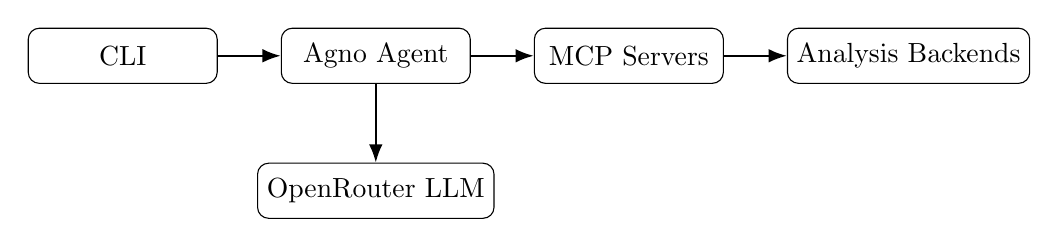
\begin{tikzpicture}[
      node distance=10mm and 8mm,
      box/.style={draw, rounded corners, align=center, minimum width=24mm, minimum height=7mm},
      line/.style={-Latex, thick}
    ]
    \node[box] (cli) {CLI};
    \node[box, right=of cli] (agent) {Agno\ Agent};
    \node[box, right=of agent] (mcp) {MCP\ Servers};
    \node[box, right=of mcp] (back) {Analysis\ Backends};
    \node[box, below=of agent] (llm) {OpenRouter\ LLM};

    \draw[line] (cli) -- (agent);
    \draw[line] (agent) -- (mcp);
    \draw[line] (mcp) -- (back);
    \draw[line] (agent) -- (llm);
  \end{tikzpicture}
\end{frame}

\begin{frame}{Tool Design Philosophy}
  \begin{itemize}
    \item Tools express analysis intent (e.g., detect crypto constants).
    \item Each tool returns structured, interpretable JSON results.
    \item Agent combines signals into a concise risk narrative.
    \item Designed for low-resource environments and reproducible runs.
  \end{itemize}
\end{frame}

\begin{frame}{Binary Analysis Coverage}
  \begin{itemize}
    \item \textbf{Static signals}: crypto constants, strings with context, imports/exports.
    \item \textbf{Heuristics}: suspicious syscalls, anti-analysis indicators.
    \item \textbf{Packing signals}: entropy analysis and optional YARA matches.
    \item \textbf{Output}: normalized JSON payload for agent summarization.
  \end{itemize}
\end{frame}

\begin{frame}{APK Analysis Coverage}
  \begin{itemize}
    \item \textbf{Permissions}: risk scoring by security-sensitive groups.
    \item \textbf{Secrets}: API keys and token patterns in resources.
    \item \textbf{Network}: URL endpoints and suspicious domains.
    \item \textbf{Obfuscation}: class name scrambling, string encryption hints.
  \end{itemize}
\end{frame}

\begin{frame}{LLM Orchestration}
  \begin{itemize}
    \item Agno agent executes tool plans and consolidates results.
    \item OpenRouter free tier keeps cost low and accessible.
    \item Fallback mode: local tools run, LLM only summarizes JSON.
  \end{itemize}
\end{frame}

\begin{frame}{Evaluation Design}
  \begin{itemize}
    \item Validate tool correctness with synthetic samples.
    \item Test CLI-only, agent-summary, and full orchestration modes.
    \item Verify resilience under rate limits and minimal installs.
  \end{itemize}
\end{frame}

\begin{frame}{Evaluation (Binary Sample)}
  \begin{itemize}
    \item Extracted \texttt{hello\_world} with surrounding byte context.
    \item No crypto constants, syscalls, or anti-analysis indicators.
    \item Entropy $\approx 3.16$ (no packing or encryption).
  \end{itemize}
  \vspace{4pt}
  \textbf{Result:} Low-risk, benign artifact.
\end{frame}

\begin{frame}{Evaluation (APK Sample)}
  \begin{itemize}
    \item Hardcoded API key pattern detected in resources.
    \item Network URLs extracted from embedded strings.
    \item No obfuscation indicators in this synthetic APK.
  \end{itemize}
  \vspace{4pt}
  \textbf{Result:} Secret exposure flagged; otherwise low-risk.
\end{frame}

\begin{frame}{Results Snapshot}
  \centering
  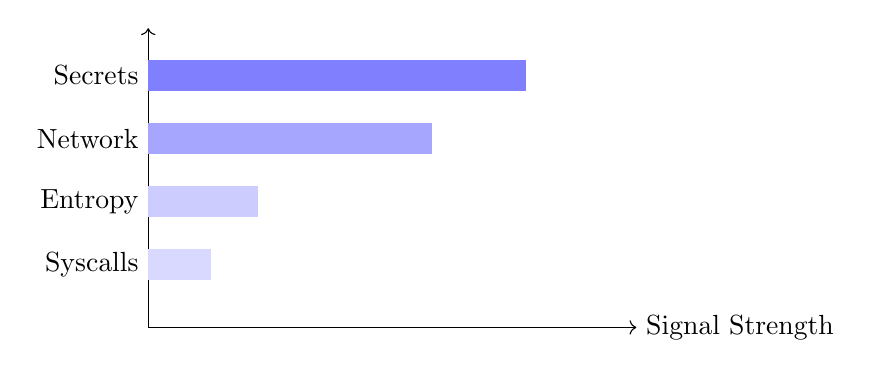
\begin{tikzpicture}
    \draw[->] (0,0) -- (6.2,0) node[right] {Signal Strength};
    \draw[->] (0,0) -- (0,3.8);
    \node[anchor=east] at (0,3.2) {Secrets};
    \node[anchor=east] at (0,2.4) {Network};
    \node[anchor=east] at (0,1.6) {Entropy};
    \node[anchor=east] at (0,0.8) {Syscalls};

    \fill[blue!50] (0,3.0) rectangle (4.8,3.4); % Secrets
    \fill[blue!35] (0,2.2) rectangle (3.6,2.6); % Network
    \fill[blue!20] (0,1.4) rectangle (1.4,1.8); % Entropy
    \fill[blue!15] (0,0.6) rectangle (0.8,1.0); % Syscalls
  \end{tikzpicture}
  \vspace{4pt}
  \small Synthetic samples show high signal for secrets/network, low for syscalls/entropy.
\end{frame}

\begin{frame}{Limitations}
  \begin{itemize}
    \item Heuristic-driven signals, not full dynamic analysis.
    \item Optional dependencies for deeper parsing (LIEF, YARA, Capstone).
    \item Free-tier LLM rate limits can restrict orchestration.
    \item Evaluation uses synthetic samples for safety and reproducibility.
  \end{itemize}
\end{frame}

\begin{frame}{Future Work}
  \begin{itemize}
    \item Graph-based similarity features inspired by Gemini.
    \item Selective unpacking and hidden-code extraction workflows.
    \item Lightweight dynamic analysis integration.
    \item Evaluation on curated malware corpora (isolated environments).
  \end{itemize}
\end{frame}

\begin{frame}{Conclusion}
  \begin{itemize}
    \item Agentic MCP workflow unifies binary and APK analysis.
    \item High-level tools provide clear, structured risk signals.
    \item Reproducible, low-cost, and ready for demo.
  \end{itemize}
\end{frame}

\end{document}
